\documentclass[sans, aspectratio=169]{beamer}
%\usepackage{eulervm}
\usepackage[scaled ]{helvet}
\usepackage[utf8]{inputenc}
\usepackage{multimedia}
\usepackage{multirow}

\usepackage[T1]{fontenc}

\usepackage{verbatim}

\usepackage{smartdiagram}

\usepackage{epigraph}

\title{
\textbf{{\LARGE Data Visualization 201}}\\
Advanced concepts \\ using OpenSource software
}

\date{LPP- \today}
\author{\underline{A. Tavant}}

%\usetheme{LPP}
\usepackage{template/beamerthemeLPP}
\setbeamertemplate{footline}[frame number]
\begin{document}

\begin{frame}
\titlepage
\end{frame}

\begin{frame}{Introduction} 
	
	\epigraph{A picture speaks a thousand words}{\textit{Napoléon 1er}}

\end{frame}

\begin{frame}{Outline} 

	\begin{itemize}
	\item Introduction : Why plotting ?
	\item Guidelines to plot {\bf WELL}
	\item Tutorial: using matplotlib
	
	\end{itemize}
\end{frame}


\begin{frame} 
	\frametitle{Introduction : Why plotting ?} 
	As scientists, we plot in order to:
	\begin{itemize}
	\item Visualize raw data (from experiment or simulation)
		\begin{itemize}
		\item<2-> \textbf{systematic} (once/twice a day)
		\item<2-> need to be \textbf{efficient} 
		\end{itemize}
	\item Present results to our supervisor/colleges
		\begin{itemize}
		\item<3-> less systematic ($\sim$ once a week)
		\item<3-> clear and consistent (easy to understand)
		\end{itemize}
	\item Present results at conference/ for thesis/ paper
		\begin{itemize}
		\item<4-> very well done ->\textbf{ many corrections}
		\item<4-> Easy to understand by a general public 
		\end{itemize}
	\end{itemize}
	
	\pause \pause \pause \pause
	{\bf Hence:} having good tools and work-flow is mandatory to be {\it efficient}
\end{frame}

\begin{frame} 
	\frametitle{Introduction : Why plotting ?} 

	\begin{columns}
	\begin{column}{0.35\linewidth}

		\begin{center}
		\smartdiagramset{back arrow disabled=true,
				text width=0.8\linewidth,
				module minimum width=2.5cm}
		\smartdiagram[flow diagram:vertical]{produce the data,
 				process the data, visualize the data}	
	    \end{center}
	\end{column}
		\pause
	\begin{column}{0.70\linewidth}
	\begin{itemize}
		\item Produce the data
			\begin{itemize}
			\item Experiment/ Simulmation
			\item Takes a lot of time
			\end{itemize}
		\item process the data
			\begin{itemize}
			\item use whatever tool you prefer (python, matlab, excel...)
			\item stock and keep both the raw and the processed data 
			\end{itemize}
		\item Visualize
			\begin{itemize}
			\item Use whatever tool you prefer
			\item not necessary the same tool as for processing
			\end{itemize}
		\end{itemize}
		
	\end{column}
		
	\end{columns}
\end{frame}

\begin{frame} 
	\frametitle{Introduction : Why plotting ?} 
	\framesubtitle{ My own tools }
	
	There is My own tools and work-flow:
	\begin{itemize}
	\item Produce data via simulation : takes \textbf{2-5 days} each
	\item store data in hierarchic format (\textbf{HDF5}, for management of extremely large and complex data collections).
	\item \textbf{Python} for processing
	\item \textbf{Matplotlib} (python library) for plotting
	\begin{itemize}
		\item \textbf{homemade} library for systematic plots
		\item generates \textbf{$\sim$25 plots and $\sim$10 movies} automatically for each plots
		\item dedicated \textbf{scripts} for presentation/paper/reports
	\end{itemize}
	\end{itemize}
	
\end{frame}


\begin{frame} 
	\frametitle{Guidelines to plot {\bf WELL}} 

		\begin{center}
		Plotting nice figures \textbf{is not magic}.\\
		\vspace{1cm}
		There is \textbf{some recipes} to help you.
		\end{center}

\end{frame}


\begin{frame} 
	\frametitle{Guidelines to plot {\bf WELL}} 

		\begin{center}
		Questions to ask yourself before even starting:\\
	\vspace{0.5cm}
		\smartdiagramset{back arrow disabled=true,
			text width=0.5\linewidth,
			module minimum width=2.5cm}
		\smartdiagram[flow diagram:vertical]{What's the message?, Who is the reader?, What's the data?}
		
		\end{center}
	
\end{frame}

\begin{frame}{Quiz time} 
	\begin{center}
	{\Large \textbf{Quiz time} : Which figure is the best ?}
	\end{center}
\end{frame}

\begin{frame}
	\begin{columns}
		\begin{column}{0.5\linewidth}
		\centering
		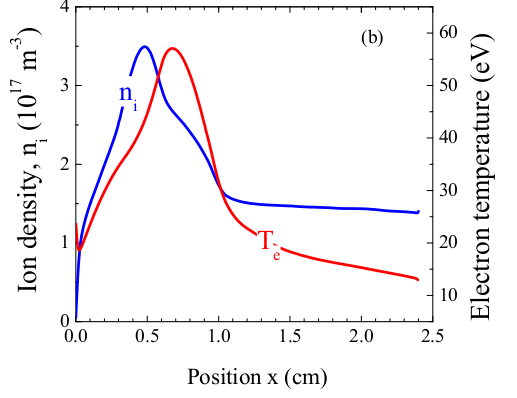
\includegraphics[width=0.8\linewidth]{proposition_from_students/I_like_antoine.png} 
		\end{column}
		\vline
		\begin{column}{0.5\linewidth}
		\centering
		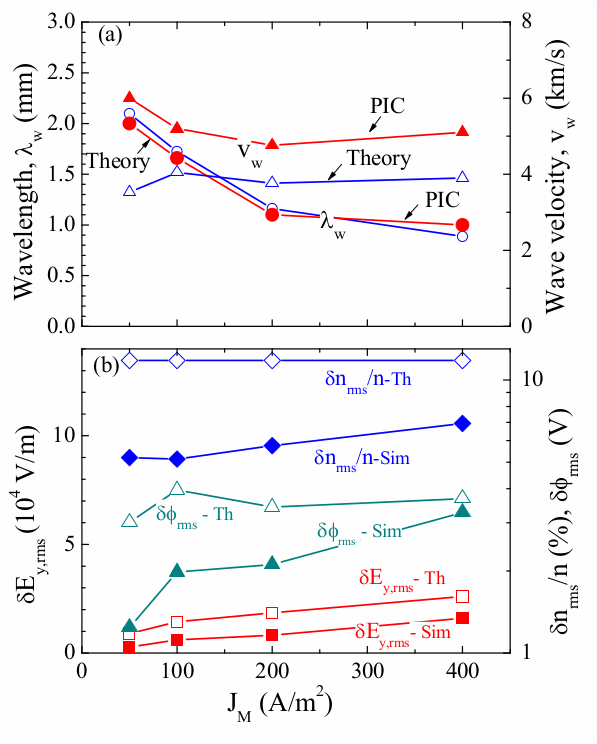
\includegraphics[width=0.8\linewidth]{proposition_from_students/I_hate_Antoine.png} 
		\end{column}
	\end{columns}
\end{frame}

\begin{frame}
	\begin{columns}
		\begin{column}{0.5\linewidth}
		\centering
		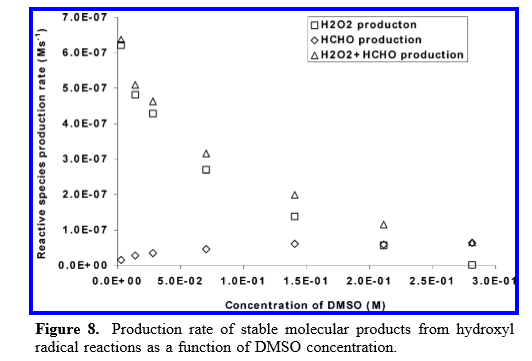
\includegraphics[width=0.8\linewidth]{proposition_from_students/I_dont_like_Constance.png} 
		\end{column}
		\vline
		\begin{column}{0.5\linewidth}
		\centering
		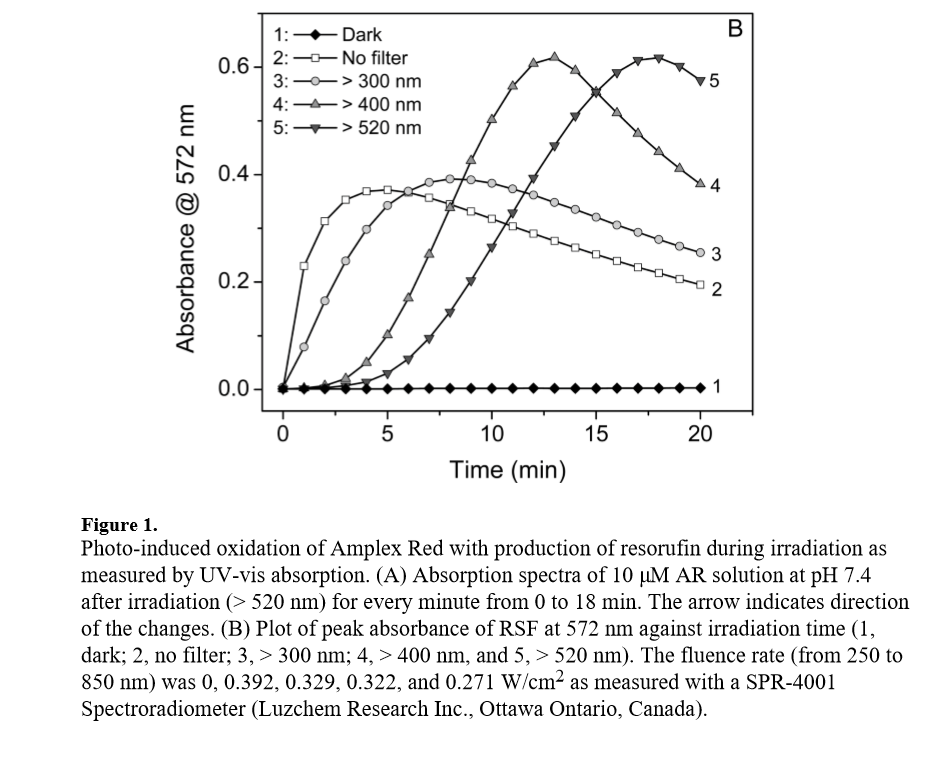
\includegraphics[width=0.8\linewidth]{proposition_from_students/I_like_Constance.png} 
		\end{column}
	\end{columns}
\end{frame}

\begin{frame}
	\begin{columns}
		\begin{column}{0.5\linewidth}
		\centering
		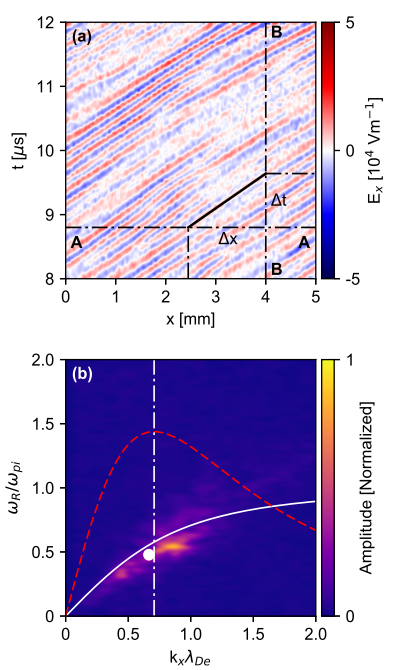
\includegraphics[width=0.8\linewidth]{proposition_from_students/I_love_Charoy.png} 
		\end{column}
		\vline
		\begin{column}{0.5\linewidth}
		\centering
		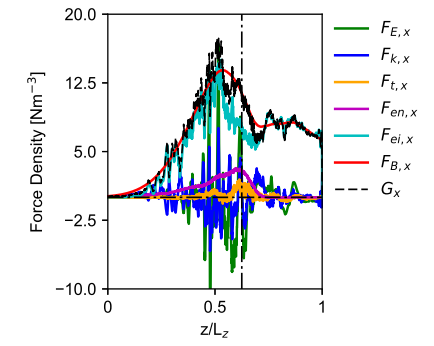
\includegraphics[width=0.8\linewidth]{proposition_from_students/I_hate_charoy.png} 
		\end{column}
	\end{columns}
	
\end{frame}

\begin{frame}
	\begin{columns}
		\begin{column}{0.5\linewidth}
		\centering
		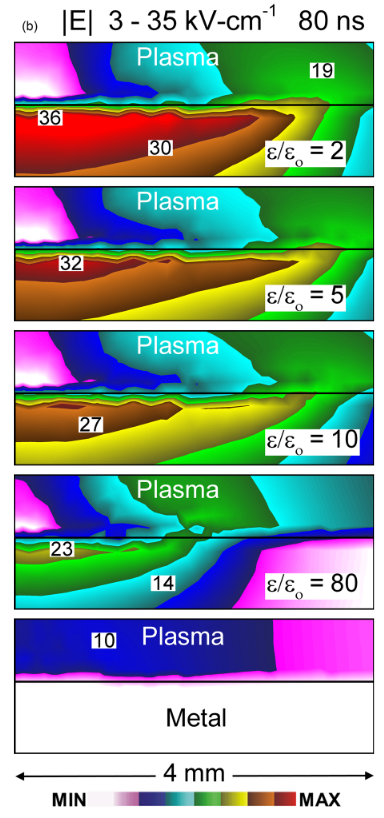
\includegraphics[width=0.8\linewidth]{proposition_from_students/uglyimage2d_pedro.png} 
		\end{column}
		\vline
		\begin{column}{0.5\linewidth}
		\centering
		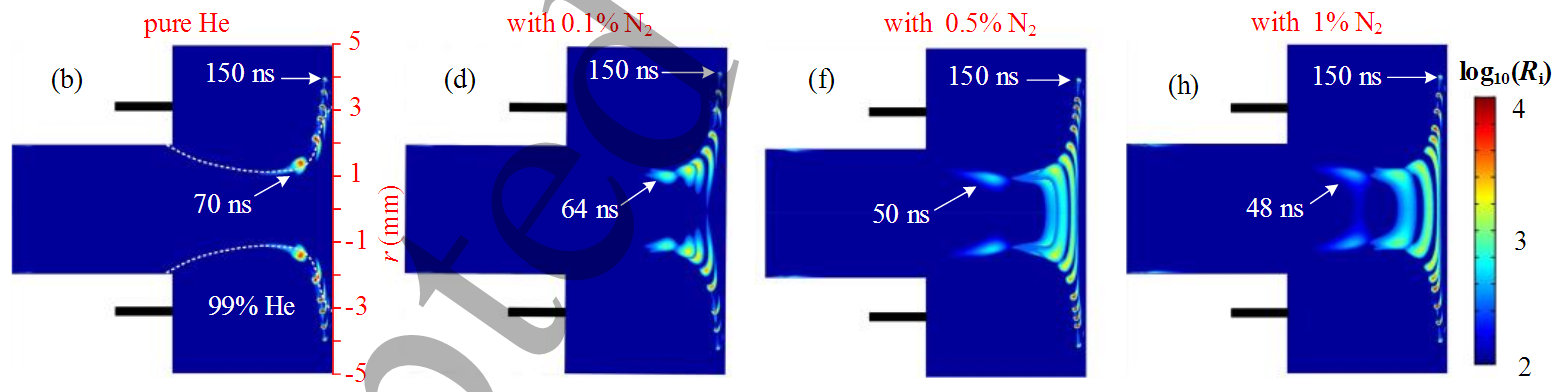
\includegraphics[width=0.8\linewidth]{proposition_from_students/niceimage2d_pedro.png} 
		\end{column}
	\end{columns}
\end{frame}

\begin{frame}
	\begin{columns}
		\begin{column}{0.5\linewidth}
		\centering
		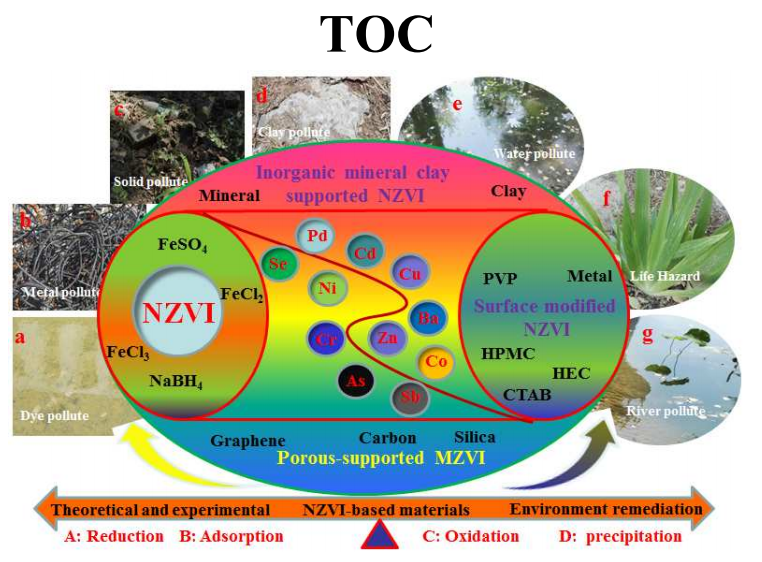
\includegraphics[width=0.8\linewidth]{proposition_from_students/I_like_Huan.png} 
		\end{column}
		\vline
		\begin{column}{0.5\linewidth}
		\centering
		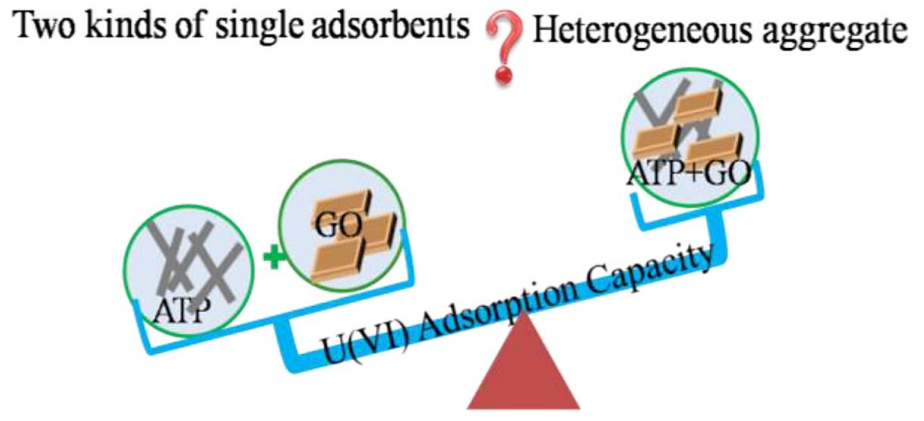
\includegraphics[width=0.8\linewidth]{proposition_from_students/I_dont_like_Huan.png} 
		\end{column}
	\end{columns}
\end{frame}

\begin{frame} 
	\frametitle{Guidelines to plot {\bf WELL}} 
	\begin{center}
	\textbf{What} is a good figure; a good plot?
	\end{center}
	
	\begin{columns}
		\begin{column}{0.5\linewidth}
		\begin{center}
		Simple to understand
		\end{center}
		\begin{itemize}
			\item<2-> simple, not too much information
			\item<2-> readable: font size and family, quality
			\item<2-> Good choice of markers, color, etc.
		\end{itemize}
		\end{column}
		\begin{column}{0.5\linewidth}
		\begin{center}
		Enjoyable to look at
		\end{center}
		\begin{itemize}
			\item<3-> simple, not too much information
			\item<3-> readable: font size and family, quality
			\item<3-> Good choice of markers, color, etc.
		\end{itemize}
		\end{column}
	\end{columns}
	\vspace{0.5cm}	
	\pause \pause \pause
	
	\begin{center}
	{\it an {\bf Enjoyable} figure will convey \textbf{more information} !} 
	\end{center}
\end{frame}

\begin{frame}
	\begin{center}
	Some Rules, not absolute and not exhaustive:\footnotemark \footnotemark \footnotemark
	\end{center}
	\begin{columns}
		\begin{column}{0.5\linewidth}
		\begin{itemize}
		\item 2-3 lines max if complex graph
		\item Think of the black-and-white prints
		\item Consistent representation 
		\item Adapt to the Support Medium
		\item Be concise (save ink)
		\item Be efficient (script, optimize)
		\item Check of typos and consistency
		\end{itemize}
		\end{column}
		\begin{column}{0.6\linewidth}
		\begin{itemize}
		\item  Do Not Trust the Defaults
		\item large font size
		\item Uses a good the font 
		\item Use vectoriel format (*.eps, *.pdf, *svg)
		\item Use Color Effectively
		\item Label axis and use units
		
		\end{itemize}
		\end{column}
	\end{columns}
	\footnotetext[1]{Ten Simple Rules for Better Figures, journals.plos.org/ploscompbiol/article?id=10.1371/journal.pcbi.1003833}
	\footnotetext[2]{Graphical Excellence in Scientific Presentations and Papers, www3.nd.edu/~pkamat/pdf/graphs.pdf}
	\footnotetext[3]{personal opinion and experience}
\end{frame}

\begin{frame}{Tutorial}

	\begin{center}
		Live example of matplotlib tips and tricks
	\end{center}	
	
	\epigraph{Never do a live example}{\textit{everyone}}
	
\end{frame}


%~~~~~~~~~~~~~~~~~~~~~~~~~
%Biblio
%~~~~~~~~~~~~~~~~~~~~~~~~~

%\begin{frame} 
%	\frametitle{Title} 
%	\framesubtitle{subtitle} 
%
%	\begin{columns}
%		\begin{column}{0.45\linewidth}
%		\end{column}
%		
%		\begin{column}{0.45\linewidth}
%		
%		\end{column}
%		
%	\end{columns}
%\end{frame}




\end{document}

